\section{图片}\label{sec:graphics}
    插入图片使用的命令是\highunderline{\textbackslash{}includegraphics[参数]\{图片路径\}},在添加包支持后,可以支持eps、png、jpg、pdf等多种格式,推荐使用png和eps两种格式的图片

    \begin{quotation}
        本手册用于说明的图片均来源于免费素材网站\href{https://pixabay.com/zh/}{pixabay},之后不再说明。        
    \end{quotation}
    \subsection{基本使用}
    \begin{texshow}
        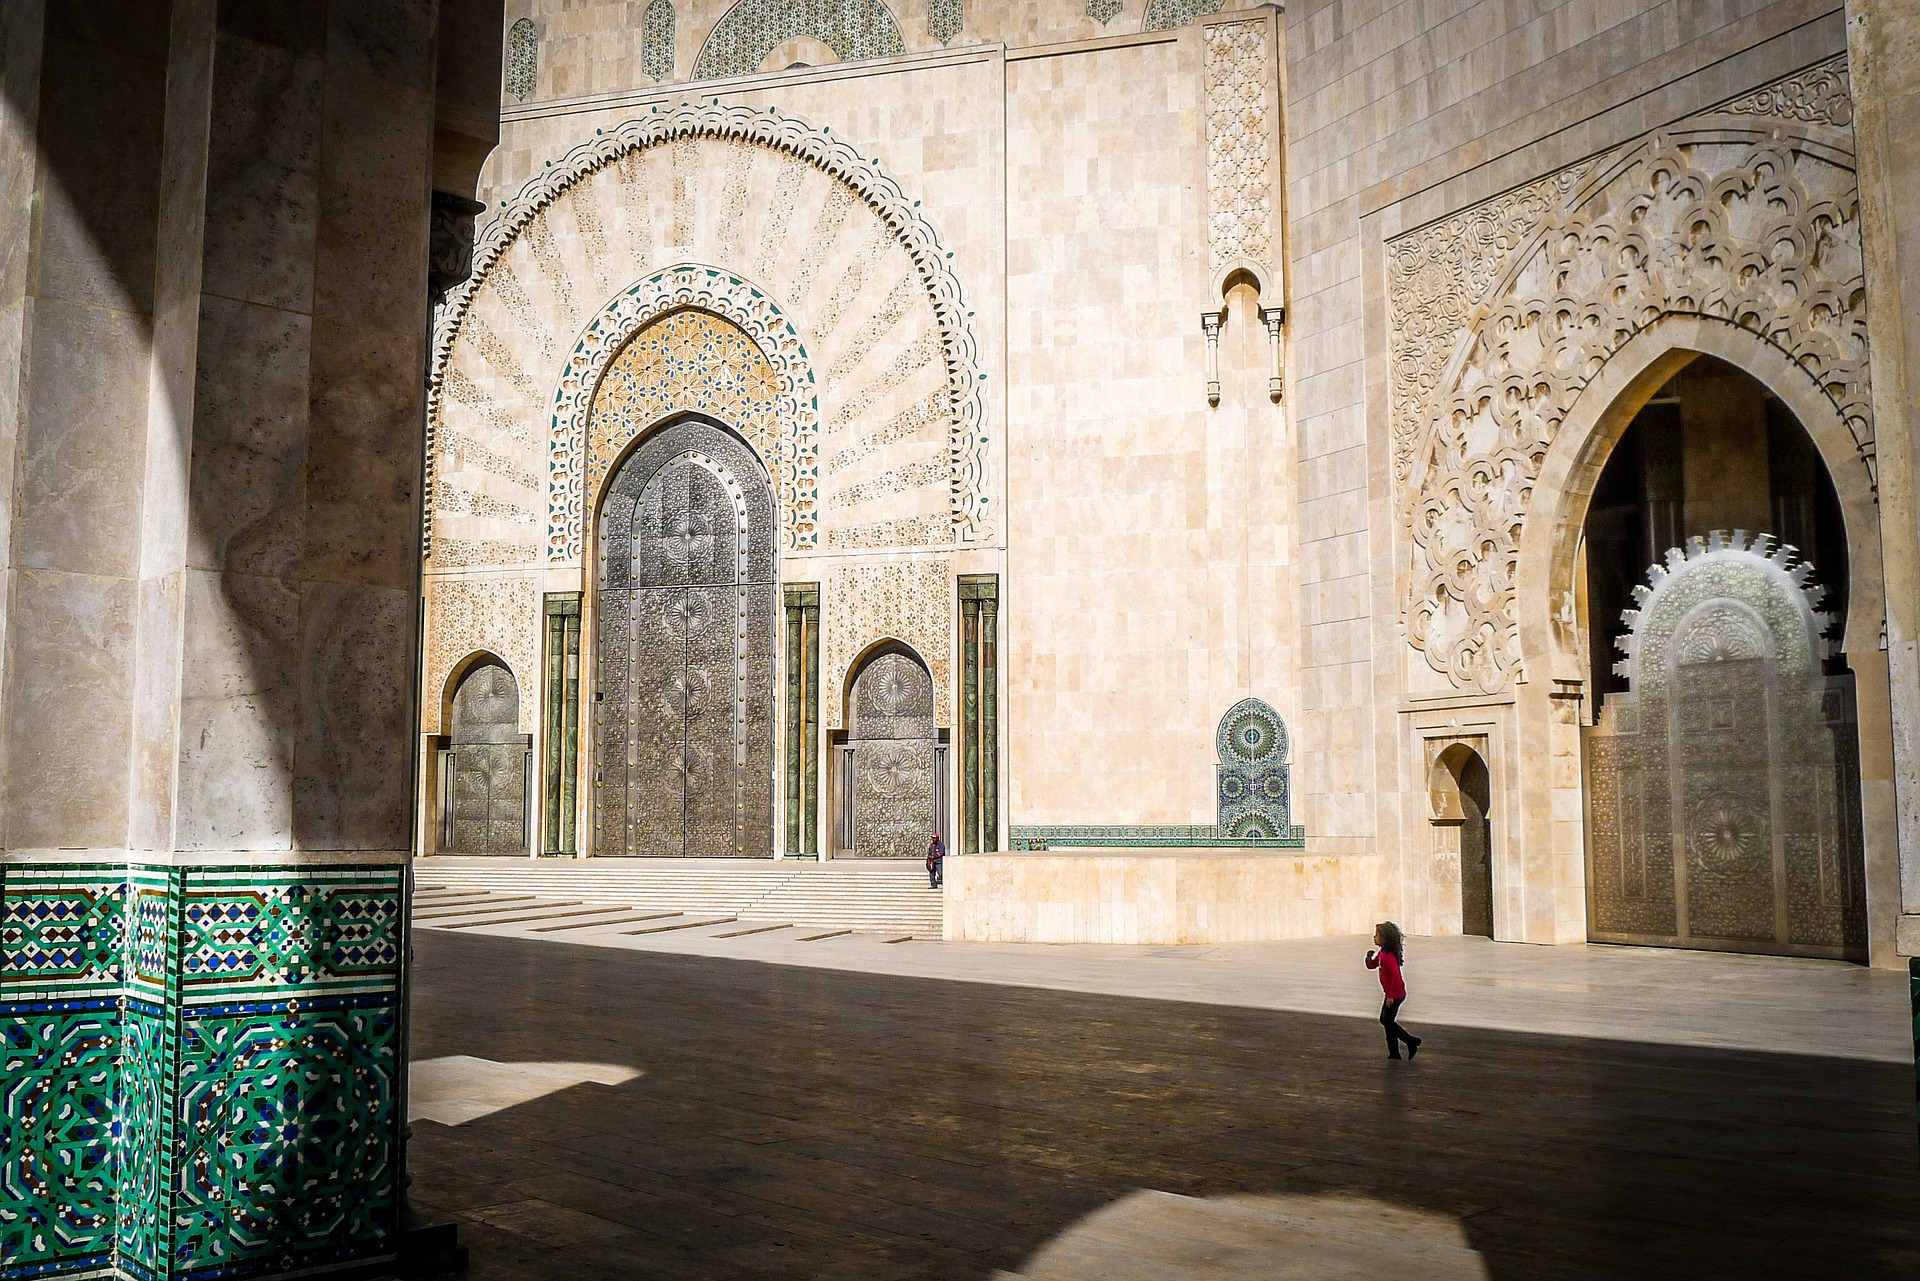
\includegraphics{contents/fig/mosque.jpg}
    \end{texshow}
    
    如上图所示,有时会会遇到图片过大的情况,因此需要加入参数调整图片的大小,因为\highunderline{\textbackslash{}columnwidth}是去掉了各种页边距后并考虑了分栏时的当前页面宽度,因此一般以该宽度作为基准调整图片大小:
    \begin{texshow}
        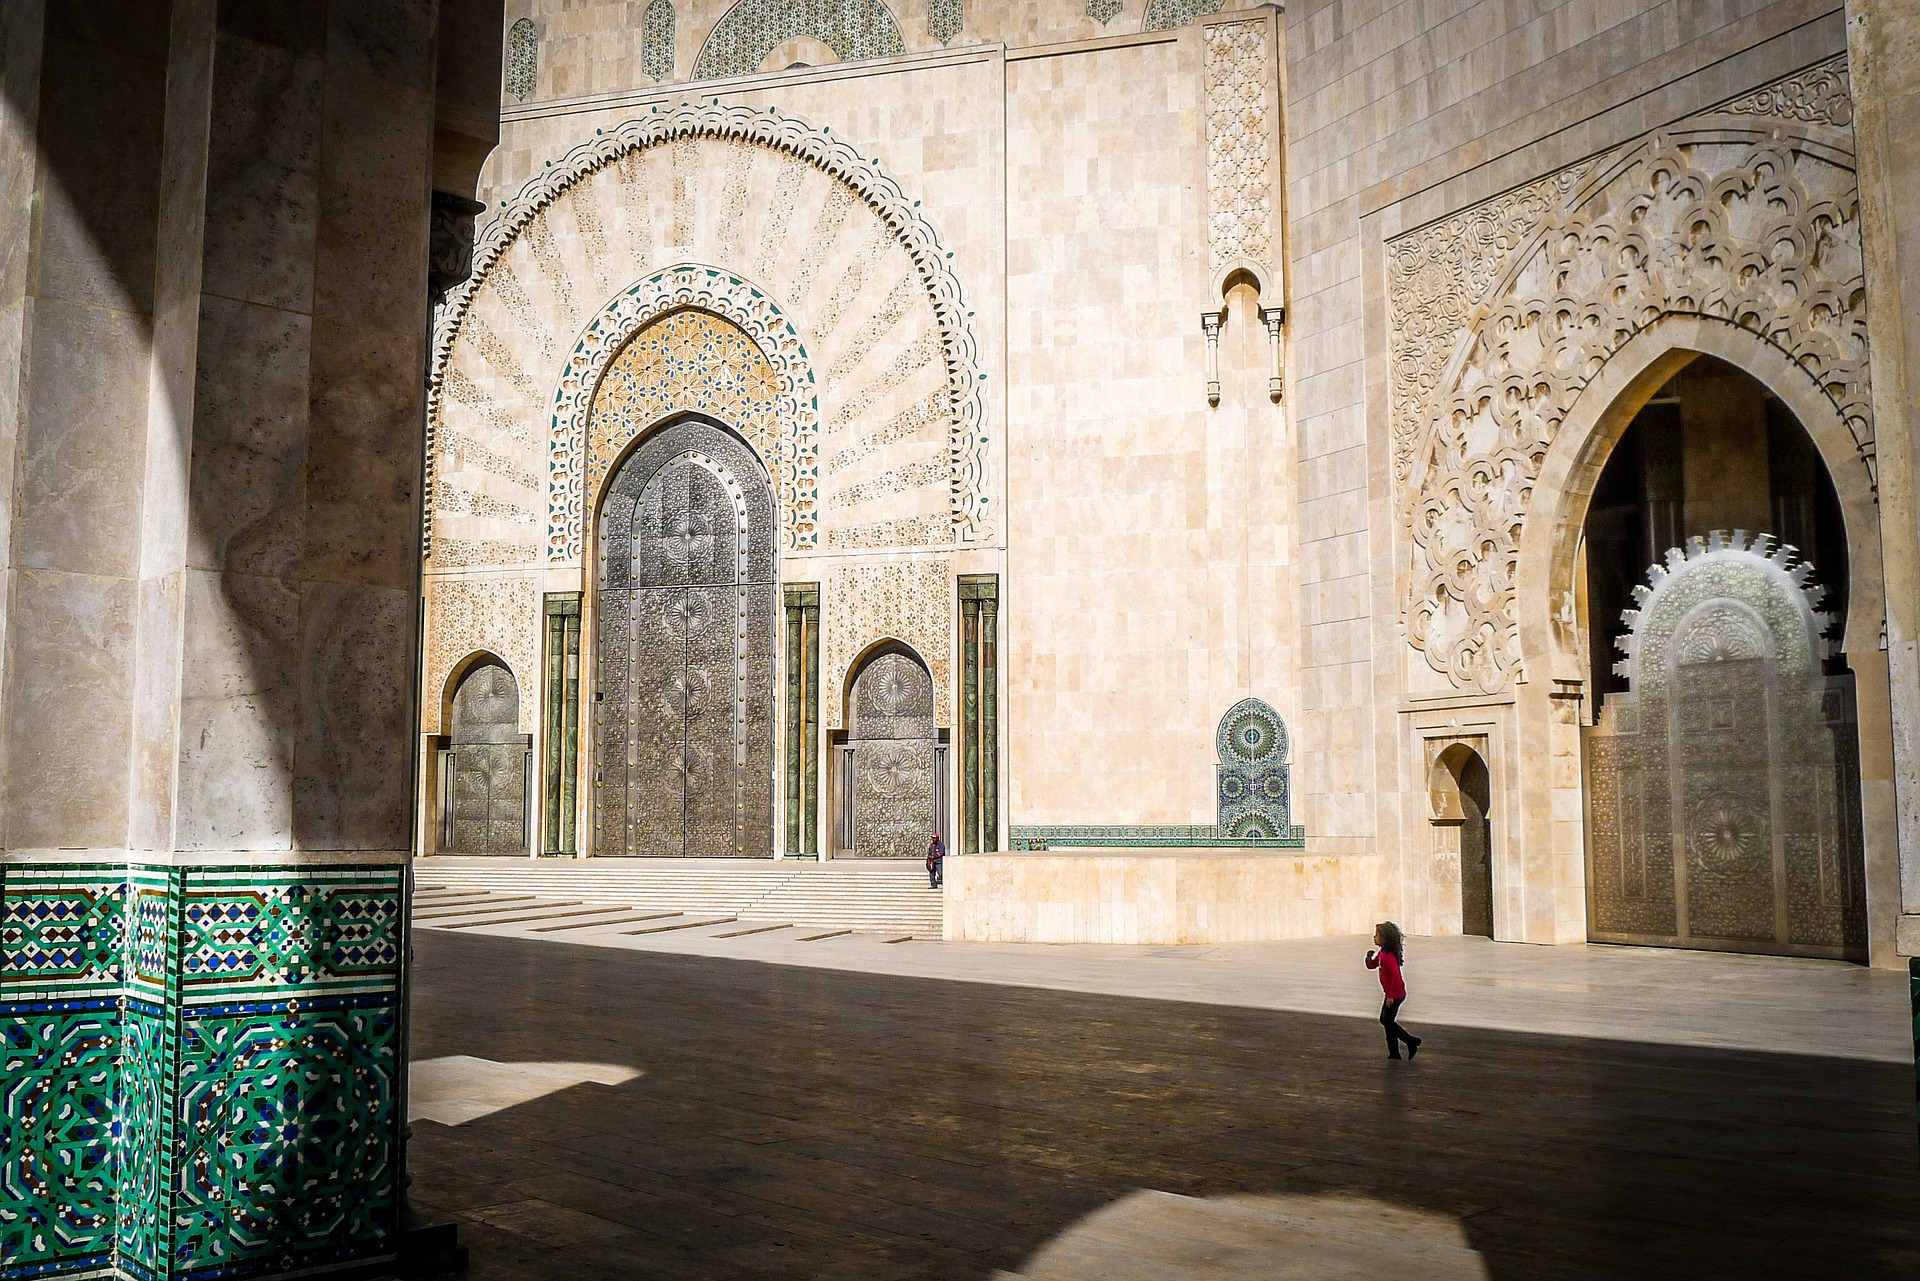
\includegraphics[width=0.5\columnwidth]{contents/fig/mosque.jpg} % 具体大小根据图片宽高比调整小数即可
    \end{texshow}

    如果是长条形图片,则可以使用\highunderline{\textbackslash{}textheight}调整图片高度的形式来适应页面。
    \begin{texshow}
        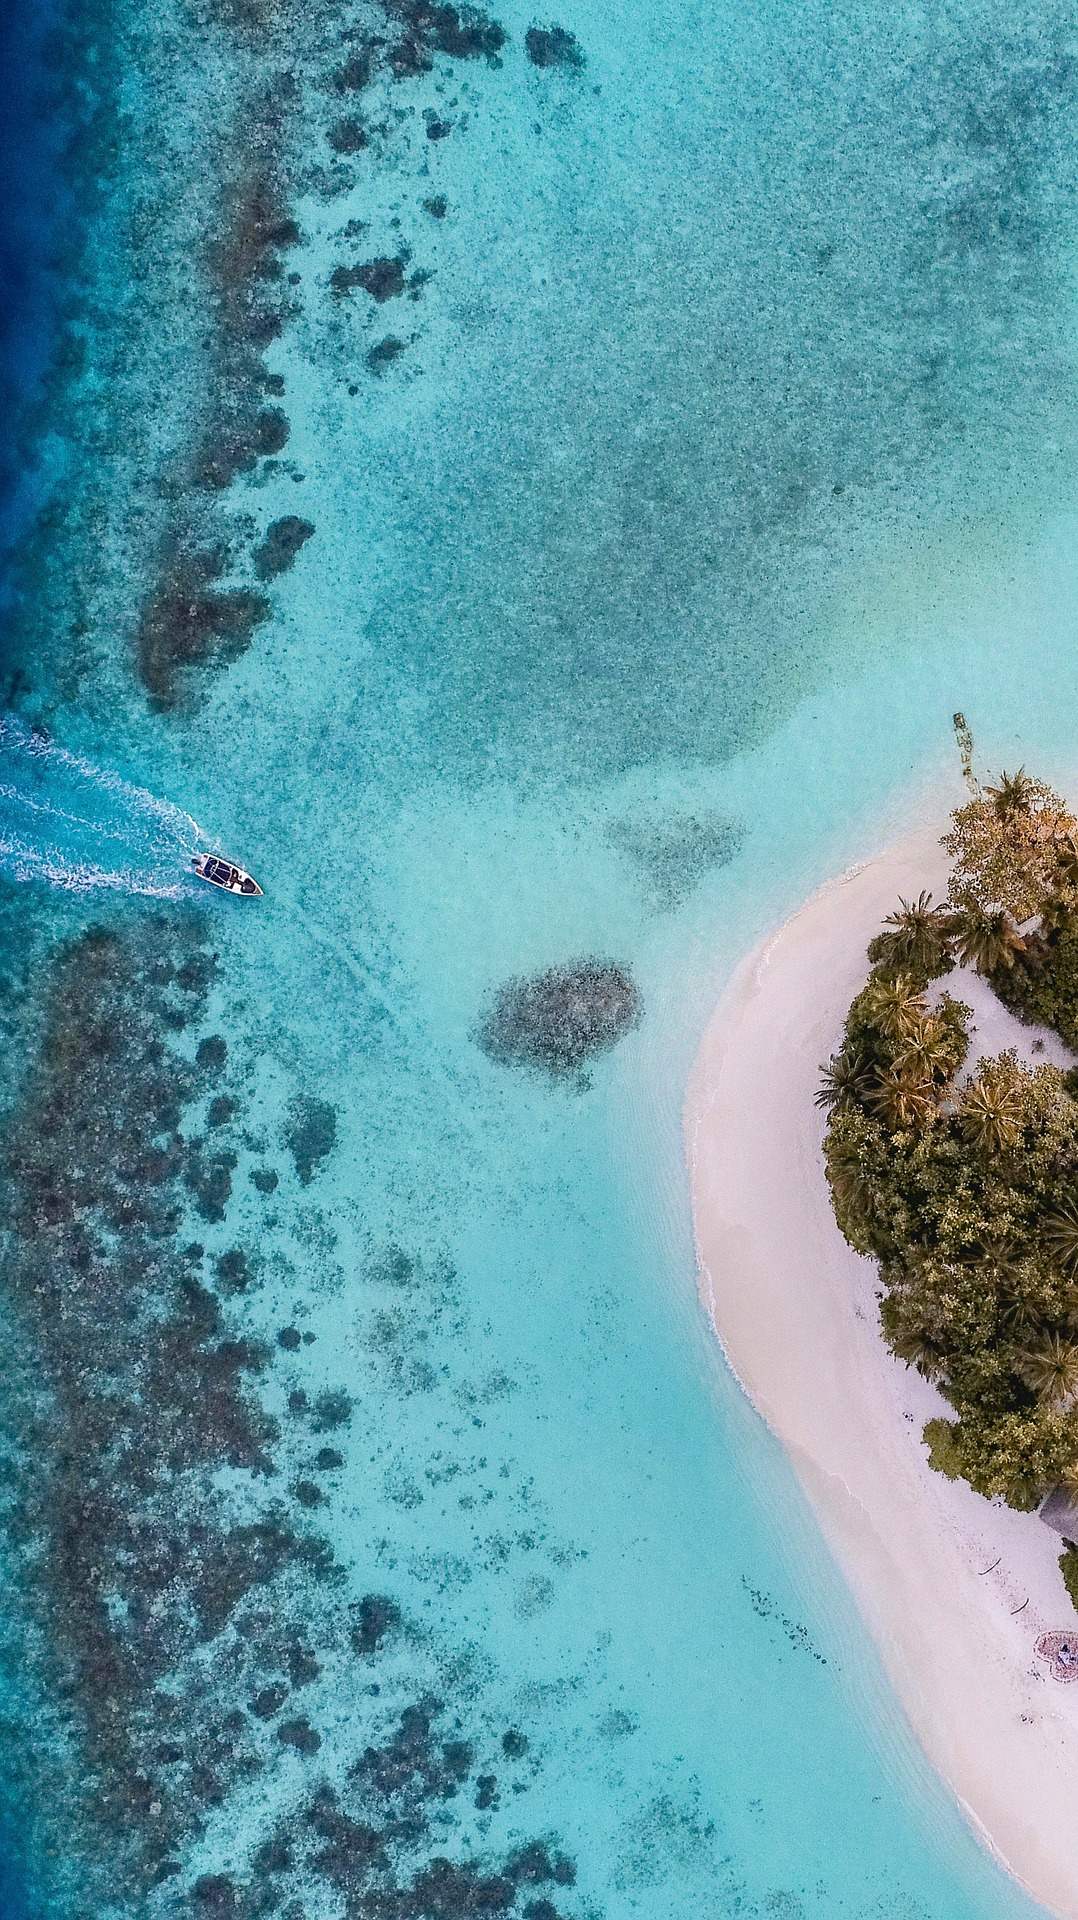
\includegraphics[height=0.4\textheight]{contents/fig/ocean.jpg}
    \end{texshow}

    注意,一般不同时调整图片长和宽,因为会导致图片失真。同时该命令还有\highunderline{scale}(缩放)参数(直接指定数字,不需要单位),但也一般不使用,因为在图片大小不统一的情况下,不便控制缩放比例。

    如果需要旋转图片,则使用\highunderline{angle}参数,直接指定数字表示度数
    \begin{texshow}
        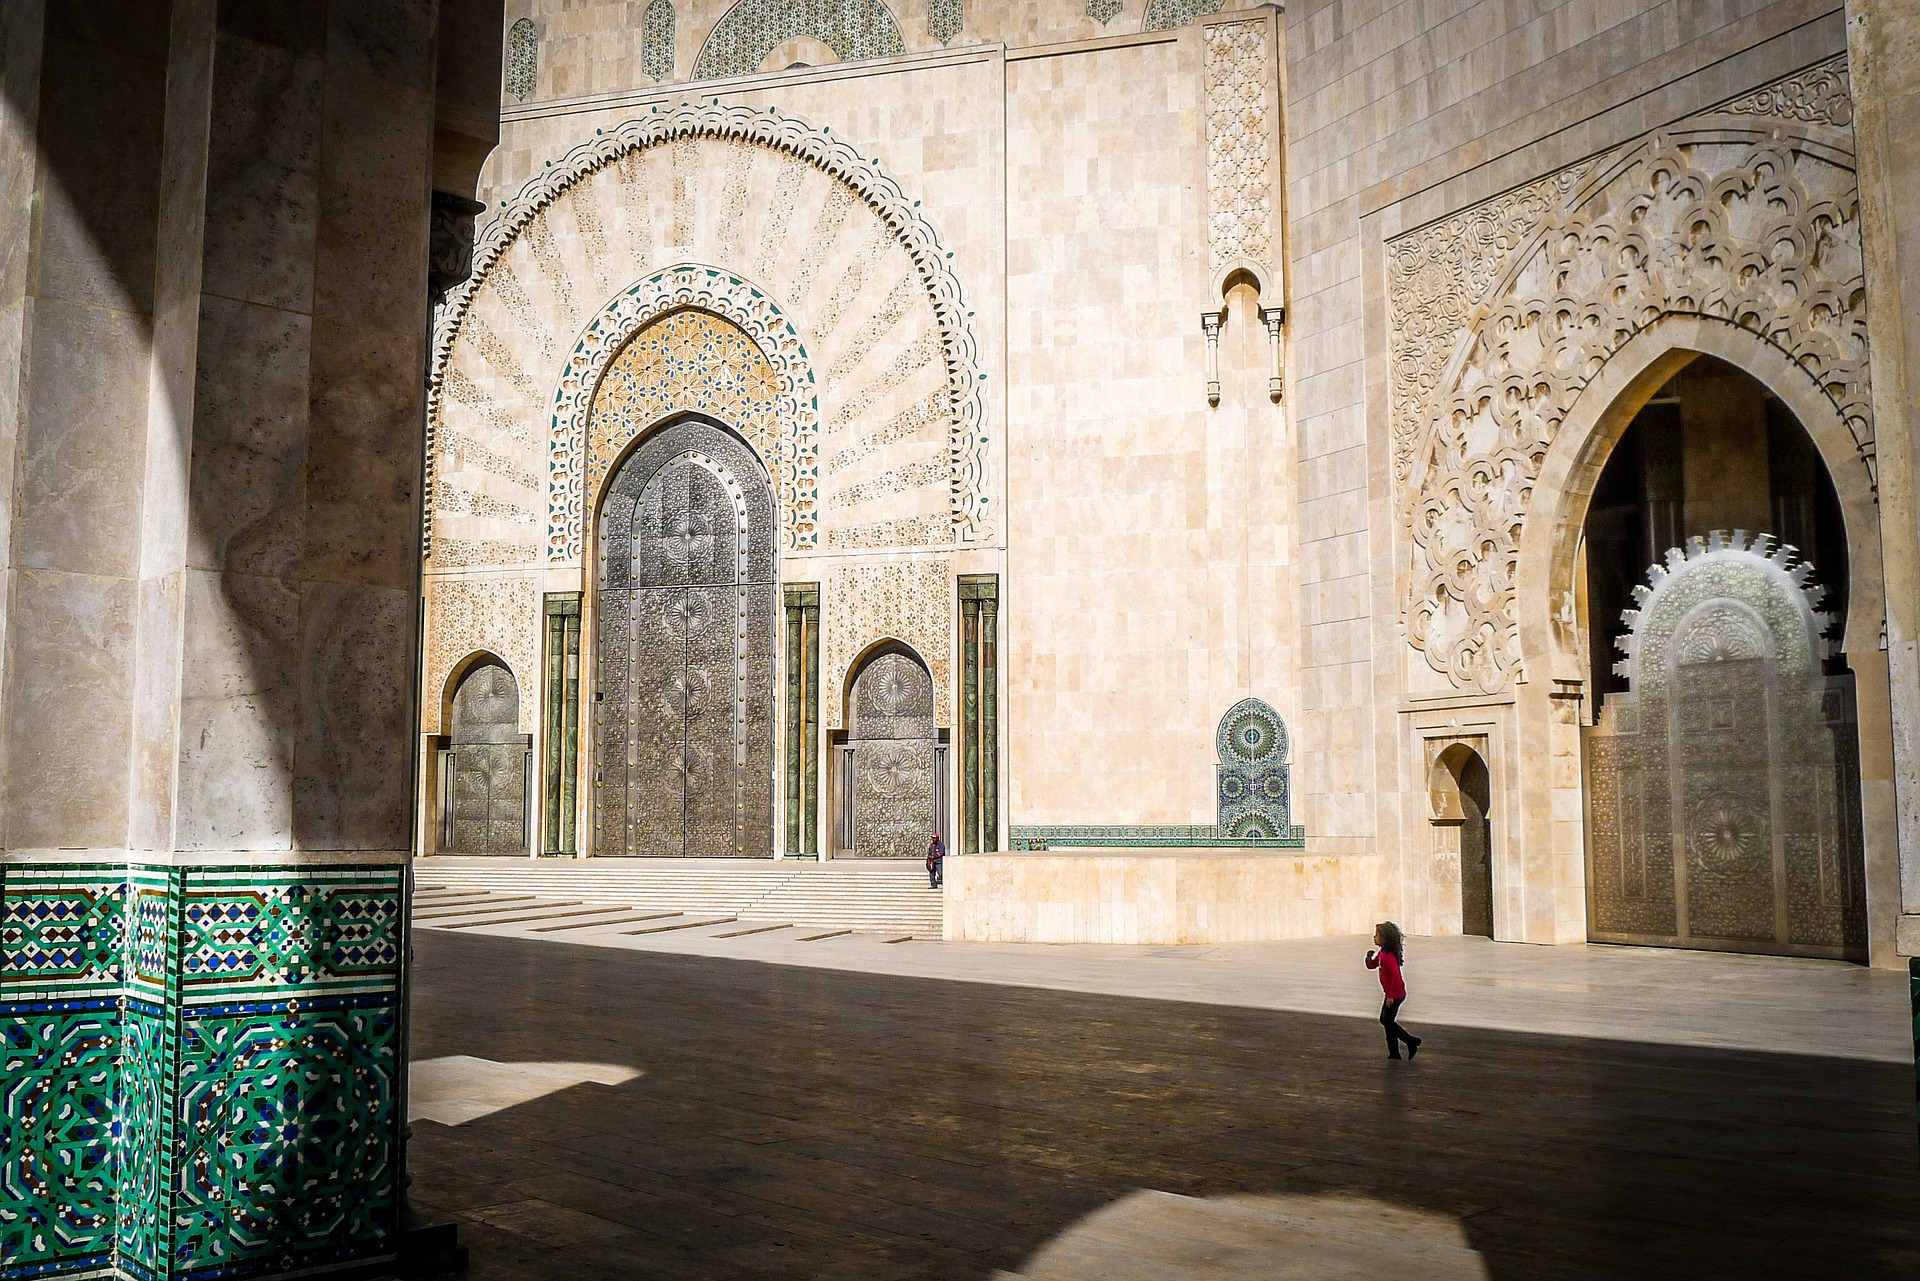
\includegraphics[width=0.3\columnwidth,angle=45]
                        {contents/fig/mosque.jpg}
        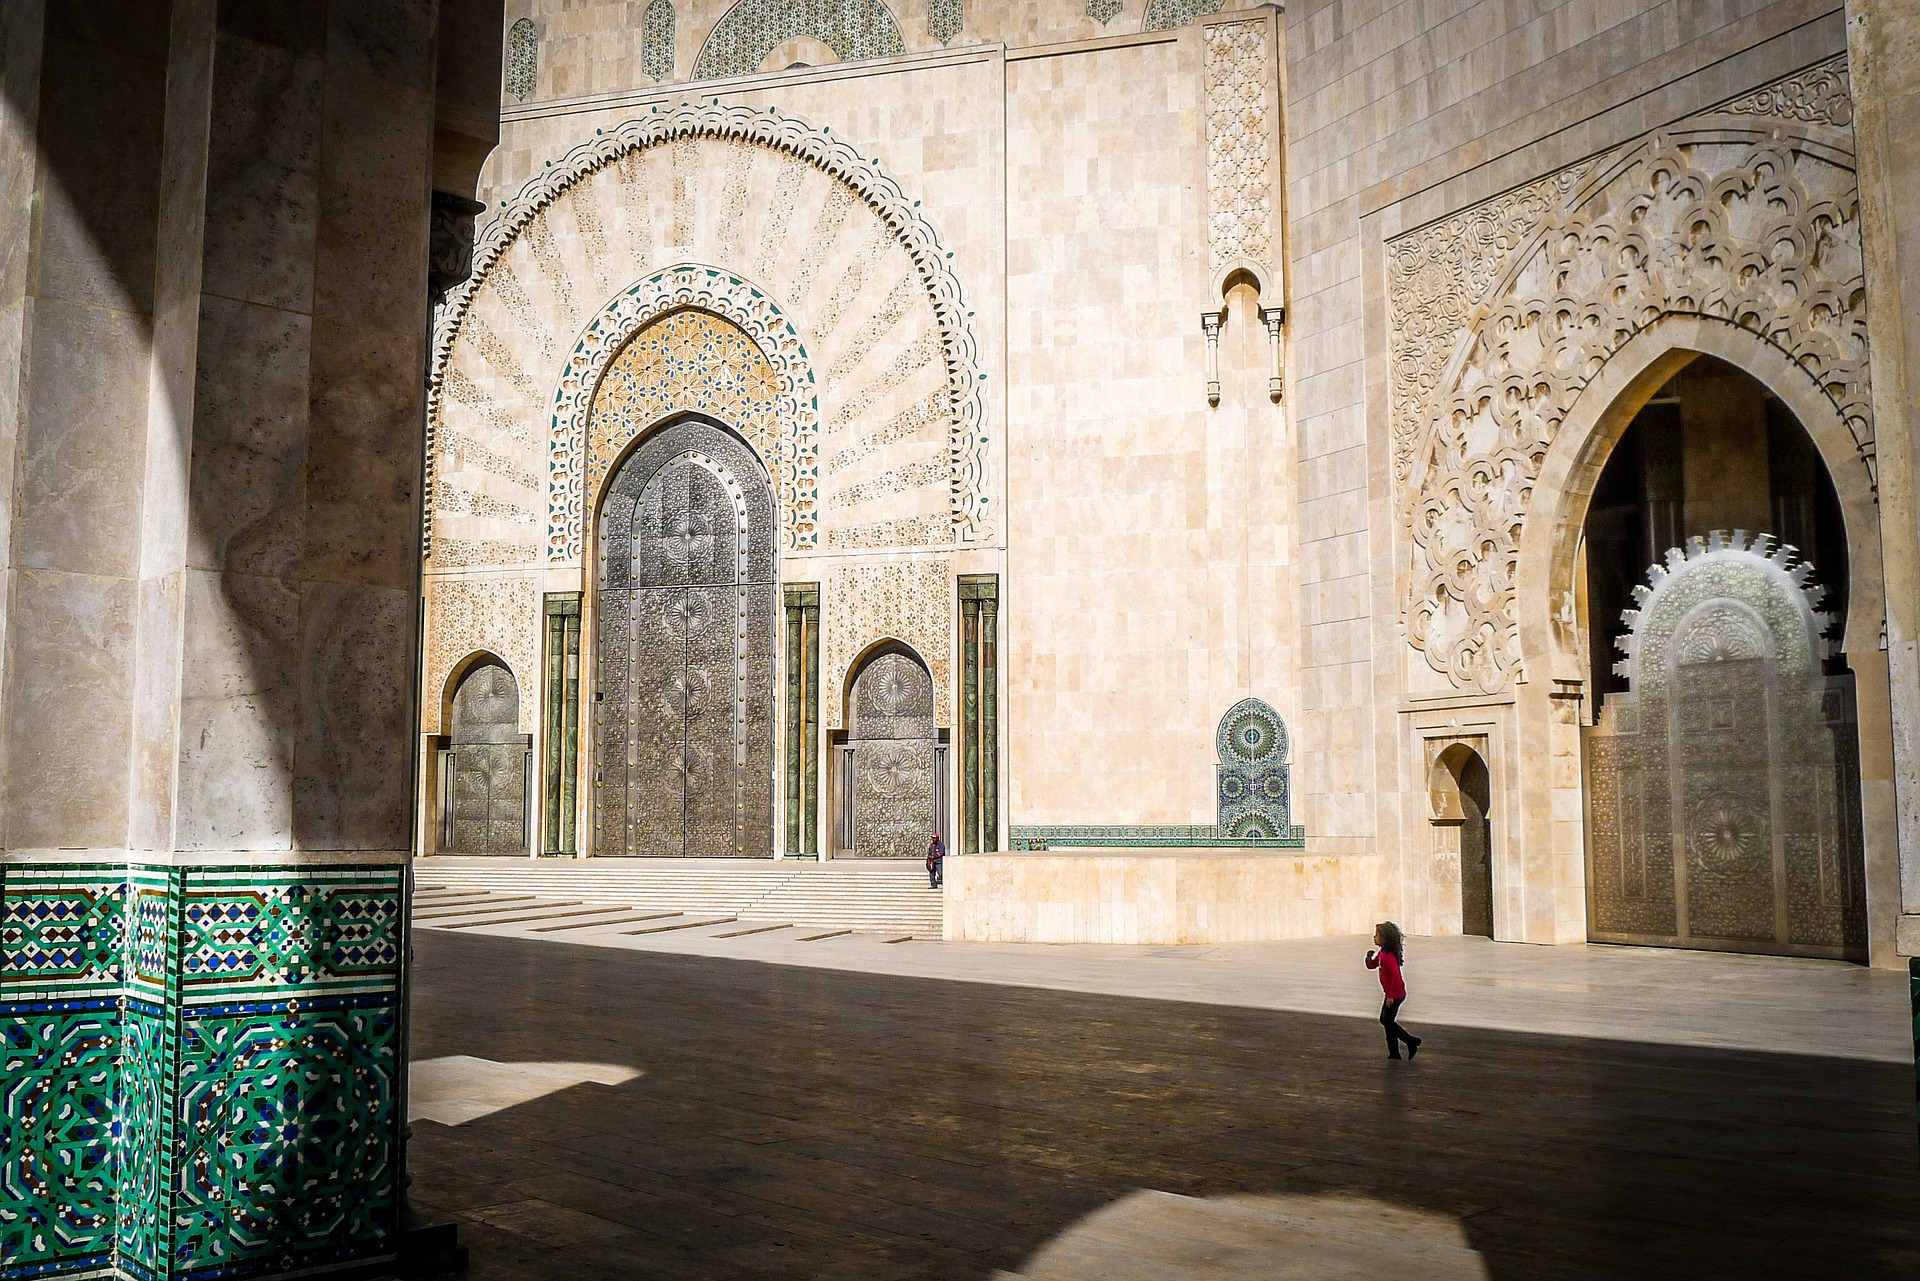
\includegraphics[width=0.3\columnwidth,angle=-45]
                        {contents/fig/mosque.jpg}
    \end{texshow}

    如果是添加PDF文档,可能会存在多页的问题,需要使用\highunderline{page}参数:

    \begin{texshow}
        \includegraphics[page=2,height=0.4\textheight]
                        {./contents/fig/section-depth.pdf}
    \end{texshow}

    如果要裁剪,则需要使用\highunderline{clip}和\highunderline{trim}参数,clip参数声明该图片需要裁剪(如果不声明则trim参数无效),trim则指明裁剪的边界:
    \begin{texshow}
        % 参数用法:trim = <left> <lower> <right> <upper>
        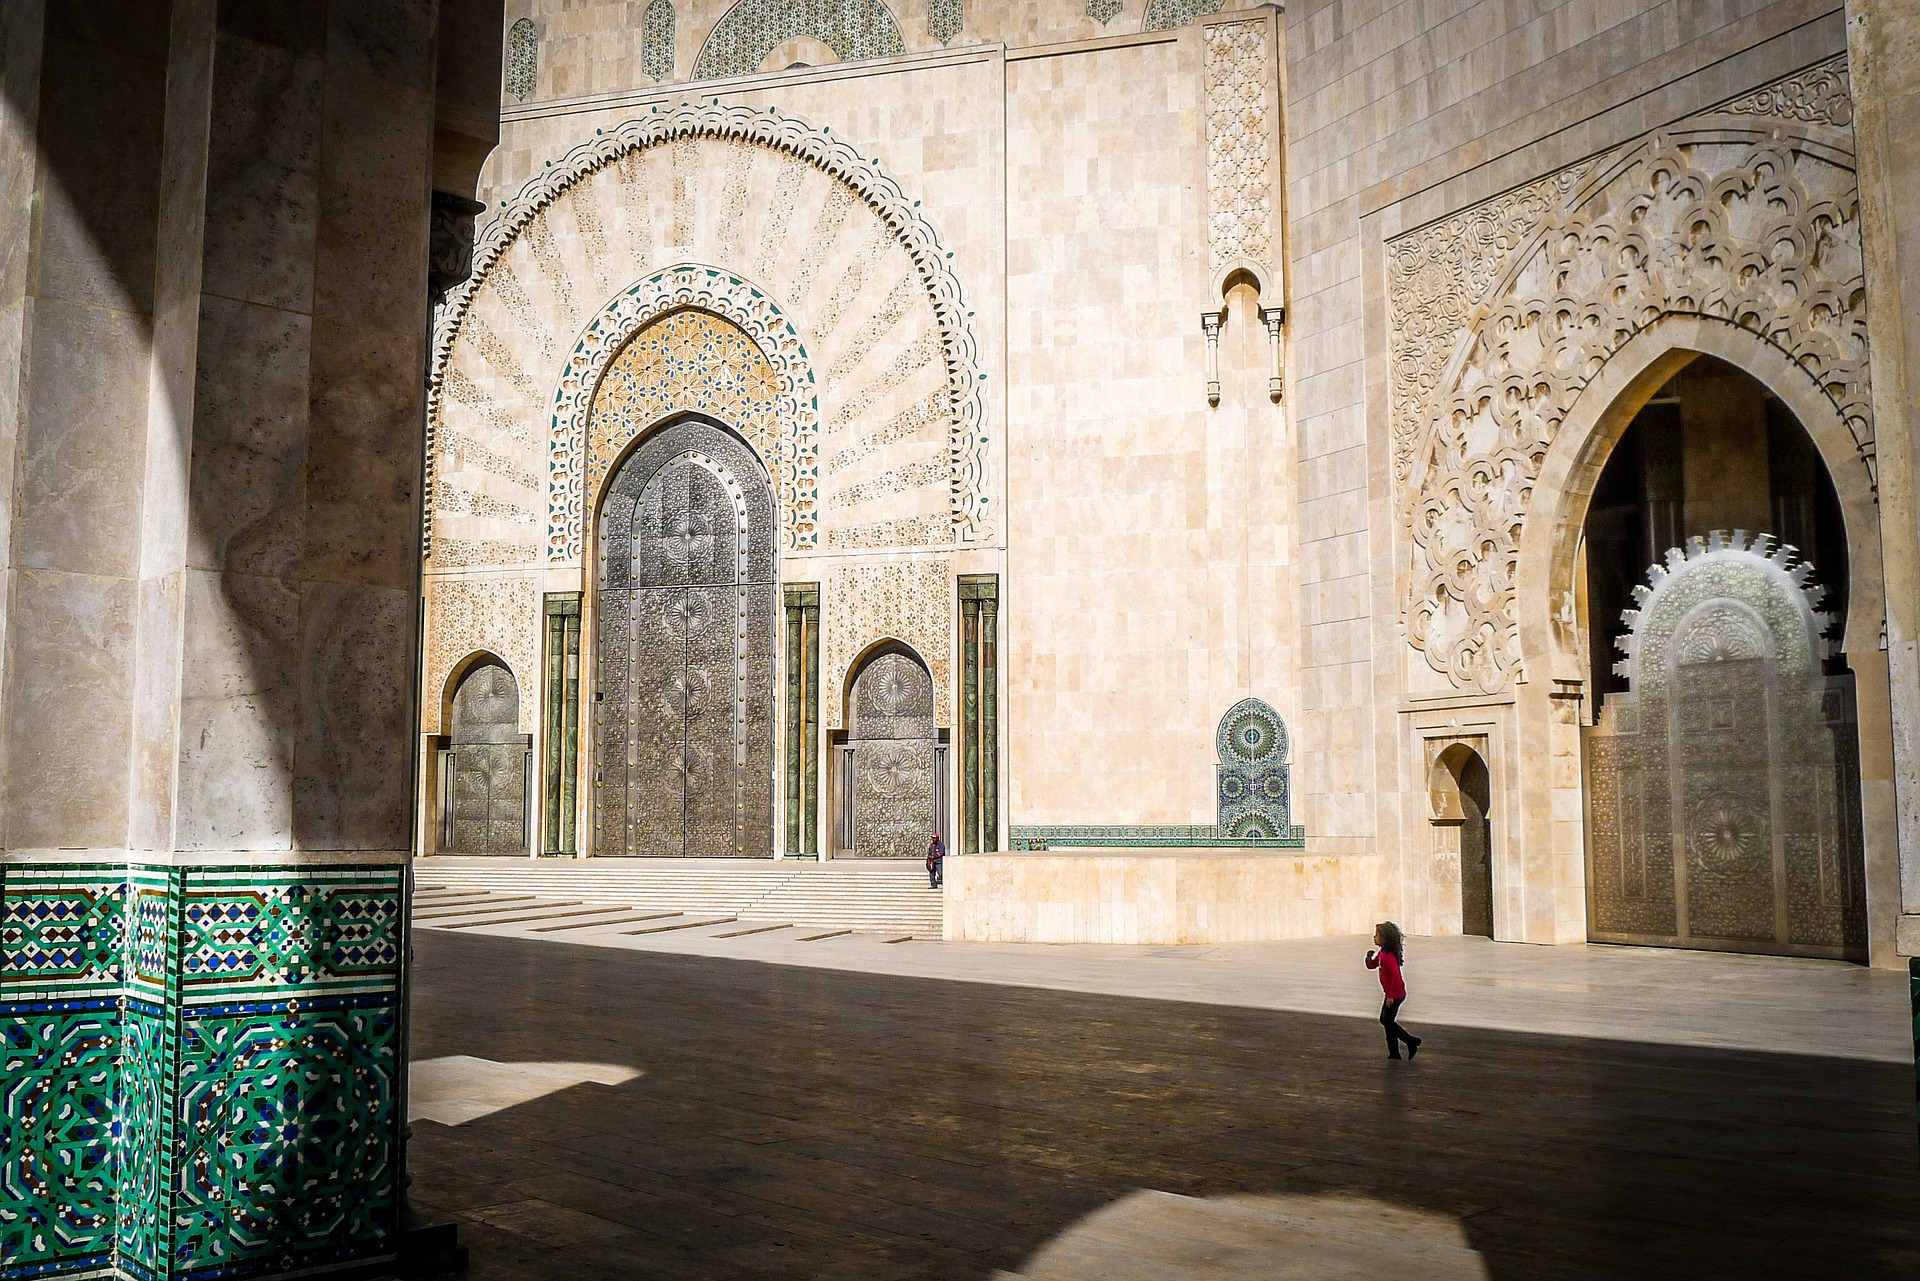
\includegraphics[clip,trim =2cm {0.4\paperheight} 2cm {0.4\paperheight},width=0.3\columnwidth]{contents/fig/mosque.jpg}\\
        \vspace{0.3\columnwidth}\\
        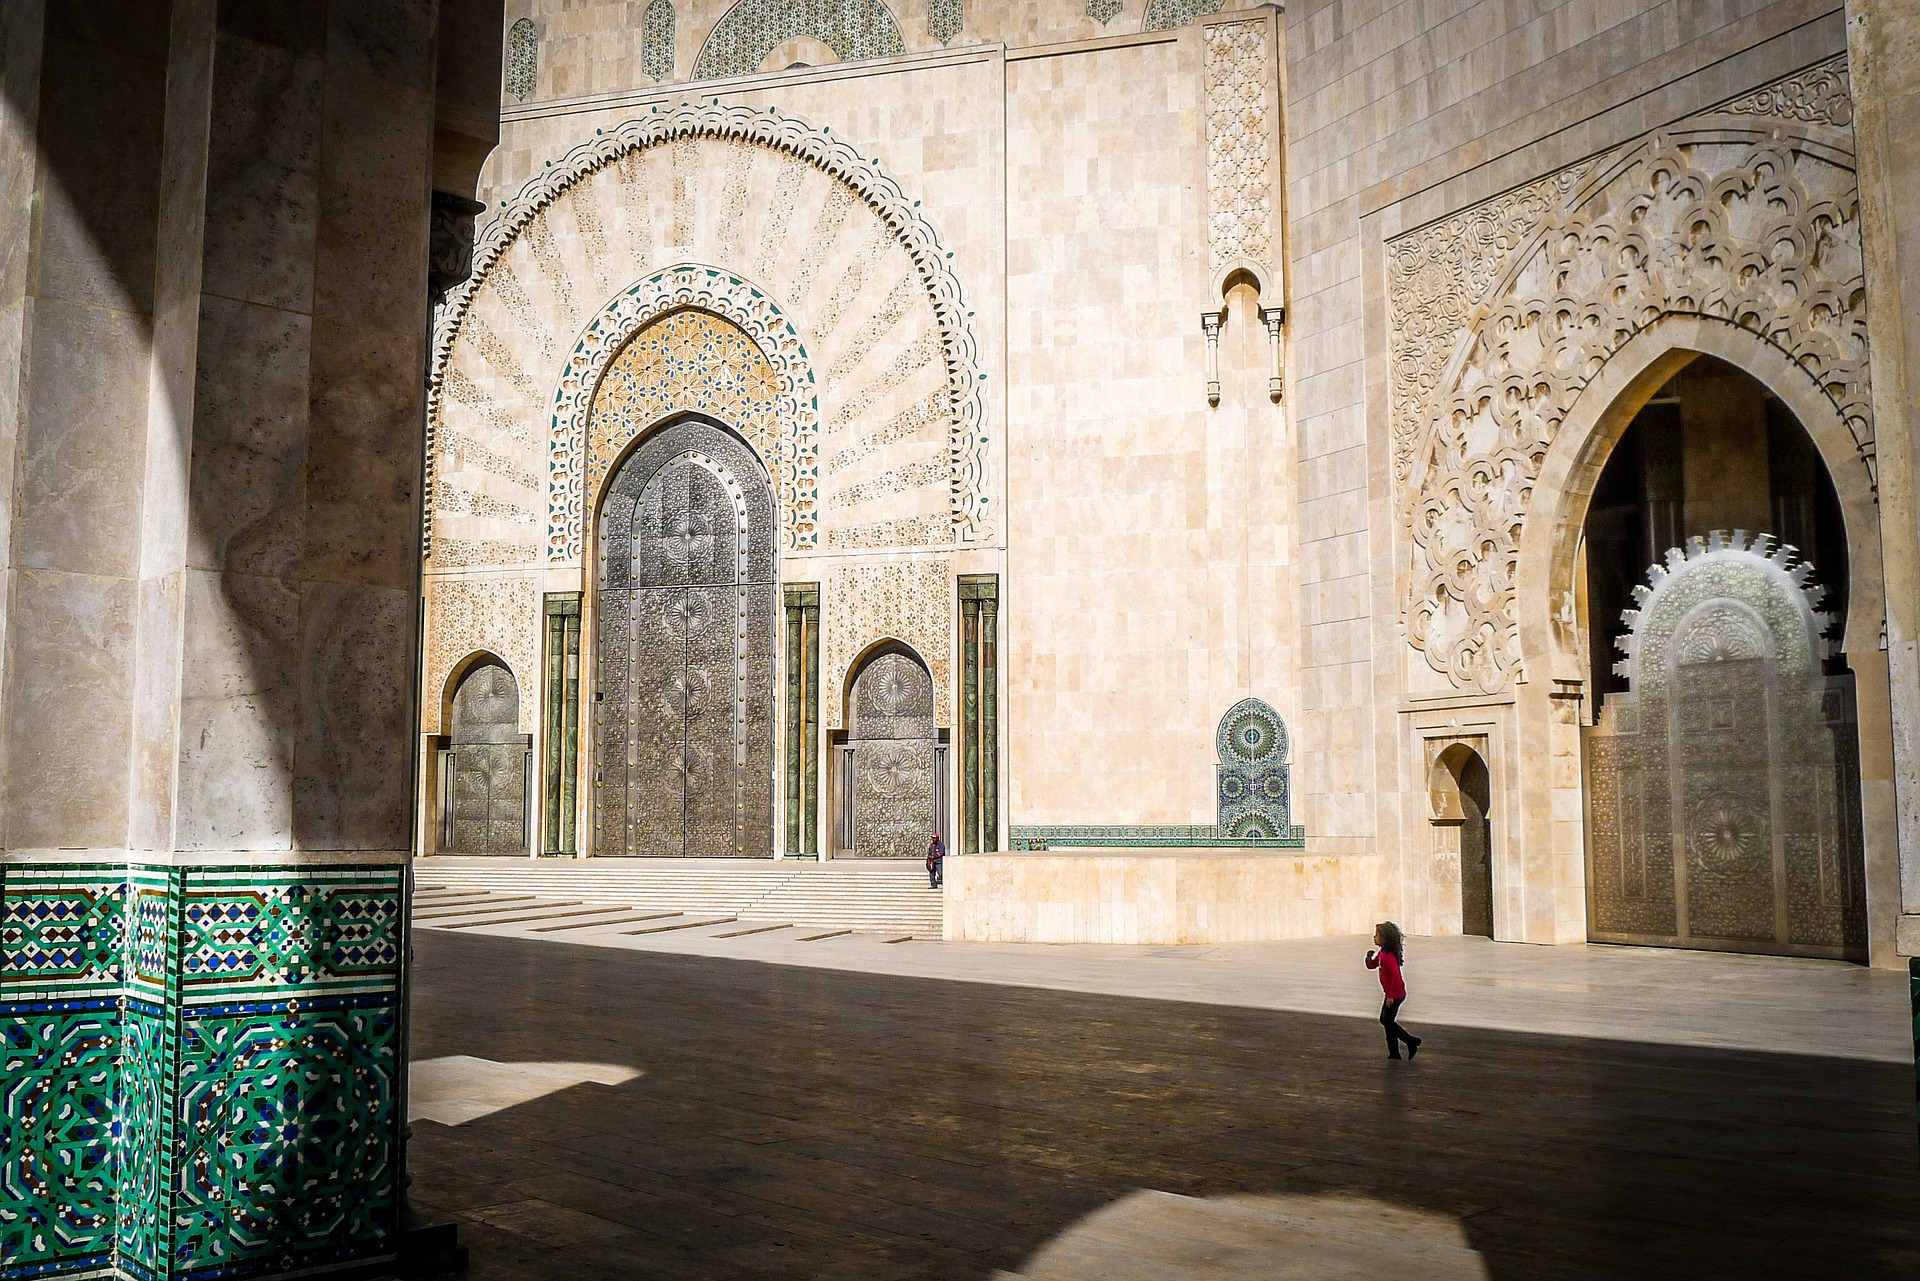
\includegraphics[width=0.3\columnwidth]{contents/fig/mosque.jpg}
    \end{texshow}
    \begin{quotation}
        注意,如果是直接指明长度,则不需要加\{...\}将长度包裹起来,如果是带有运算性质的长度,那么则需要用\{...\}将长度包裹起来,否则无法识别。
    \end{quotation}

    \subsection{指明图片路径}
    \highunderline{\textbackslash{}includegraphics}命令支持相对路径(\LaTeX{}编译时路径)和绝对路径两种路径,但即使是相对路径,有时也会因为更改而导致目录失效,因此可以以下命令指明图片目录,从而在插入图片时候只需要添加图片名字即可。

    \begin{texcode}
        \graphicspath{{./}{./contents/}{./contents/fig/}}%设置图片可能存在的路径
    \end{texcode}

    设置后\LaTeX{}编译时会自动寻找目录下的图片。

    \subsection{图片优先级读取}
    如果不加扩展名,编译时会依次寻找同名且为图片格式后缀的文件,在序言区声明以下内容可以更改其优先级。
    \begin{texcode}
        \DeclareGraphicsExtensions{.eps,.png,.jpg}%对于同名图片的优先顺序调用
    \end{texcode}

    \subsection{添加图片说明}
    参考\Ref{sub:figure}一节对\highunderline{Figure}环境的说明。

    \subsection{Tikz绘图}
    \LaTeX{}内内置了绘图方法,可以直接绘制出矢量图,\href{http://www.texample.net/tikz/examples/all/}{TikZ and PGF examples}网站上提供了大量精美(或复杂)的Tikz绘图示例:
    \begin{figure}[H]
       \centering
       \includegraphics[width=0.8\textwidth]{\figpath{tikzexample.png}}
       \caption{TikZ and PGF examples网站截图}
       \label{fig:tikzexample.png}
    \end{figure}
    使用Tikz的一个示例如下:
    \begin{texshow}
        \begin{tikzpicture} 
            \draw[step=1,color=gray!40] (-2,-2) grid (2,2); 
            \draw[->] (-3,0) -- (3,0);
            \draw[->] (0,-3) -- (0,3); 
            \draw (0,0) circle (1);  
        \end{tikzpicture}     
    \end{texshow}
    理论上Tikz可以绘制出你想要的任何图片,但是实际上由于该宏包过于复杂,除了技术狂魔外我不推荐直接使用内置的Tikz宏包来绘制矢量图...而是通过其他的手段(如Adobe Illustrator,Matplotlib)导出矢量图后以图片的形式添加,因此这里仅仅简单的介绍一下Tikz,具体的使用略。

